\chapter{SW and HW Implementation}
\label{cha:software and hardware implementation}
The overall system will work as follows:\newline 
1. The microphones capture the user voice and save their in the buffer\newline
2. When the buffers are full in the respective devices, the KWS action performing device, will process the input in Syntiant Pipeline, meanwhile SV performing device will wait for a response\newline
3. The KWS routine finishes and it communicates the classification output to SV device via SPI\newline
4. The SV according to the output if it is a class computes the Syntiant pipeline\newline
5. After d-vector extraction, it compares the result obtained with the reference vectors of the corresponding word, limiting unnecessary comparisons.\newline\newline
The possible outputs of the system are:\newline
• No word recognized, both devices return sampling\newline
• Is recognized a word, but the user is not enrolled for that word\newline
• Is recognized a word and the user is enrolled\newline
According to these different outputs, the programmer will be free to perform a connected action.\newline
This thesis, at first, was developed considering the system implementation on two Syntiant NDP101 devices with the objective in creating a multi-model system. Ultimately due to a NDA was not possible to deploy, the overall idea will be presented as if the access to the SDK was granted.
A multi-model system consists in having a uniformly signal processing with an appropriate reshape and MFE block processing by a NDP101 and then only then the result will be parsed to the other device to perform a different model action.
During the dissertation of the methodology used in software pipeline, there were used two different approaches:\newline\newline
• Simulation on computer (Software Approach) - Created to verify system pipeline correctness before deployment. It does not use any hardware component, except for the microphone integrated in the computer. It shows the behavior using pure C code and saving the models in header\newline
• Inference on MCU (Software + Hardware Approach) - Actually application deployment, which require handle of hardware components. In this case, the models are uploaded in binary files, but each one on a different MCU, not like the simulation, which had all accessible by the same compiler. The hardware and the communication (SPI) had to be managed, but the other phases are the same edited in C in simulation.\newline
\begin{center}
    \centering
    \begin{figure}[!h]
        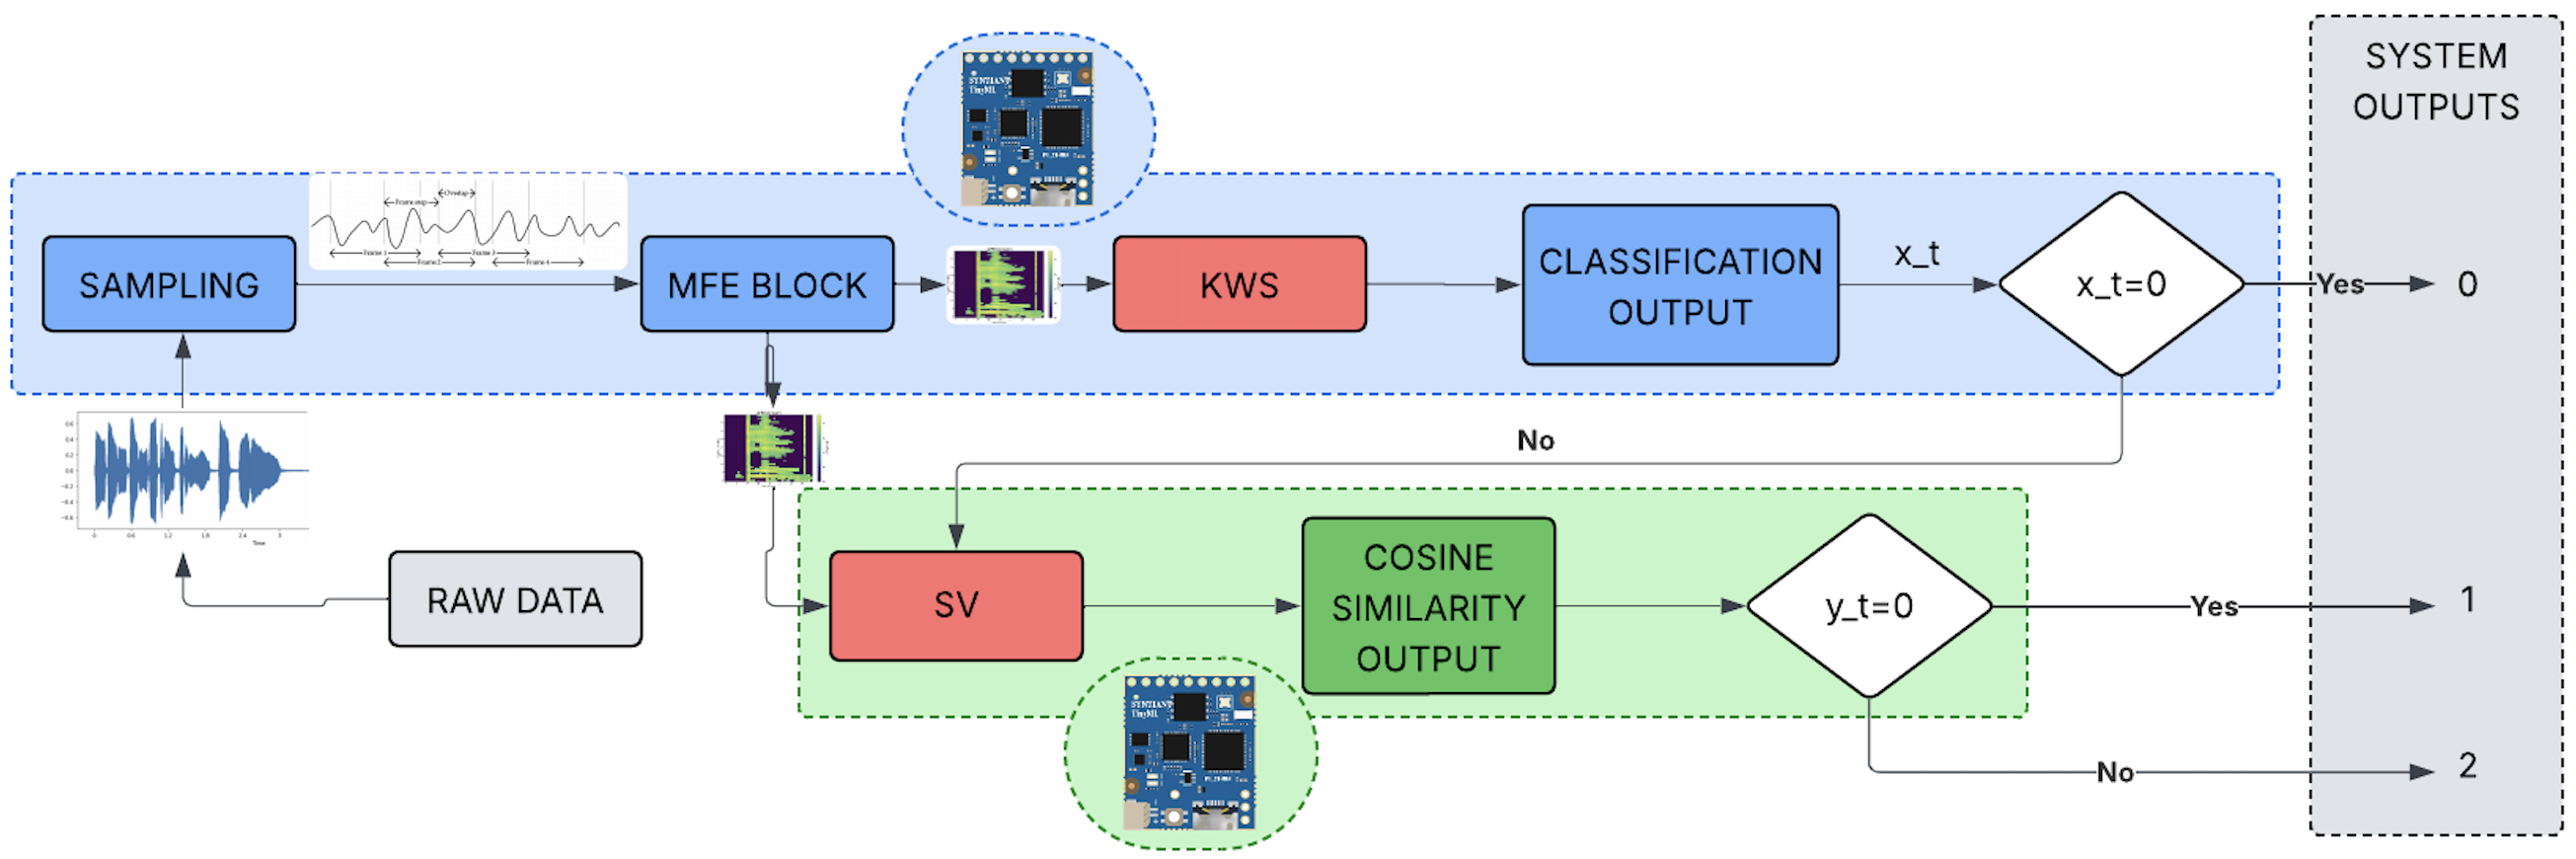
\includegraphics[width=1.0\textwidth]{images/4.01 Software Pipeline.png}
        \caption{Software Pipeline}
    \end{figure}
\end{center}
\section{Software Pipeline}
\label{sec:sw pipeline}
The system was developed in simulation and in validation using a simulation software approach, instead in inference only the code logic inside the single NDP101 was developed. In this section, we will talk about:\newline
• Signal Capture (Simulation)\newline
• MFE Block Generation and Processing (Simulation+Inference\footnotemark{}\footnotetext{According to the inability to perform the complete pipeline on NDP101, has introduced before was used for validation on MCU a STM32, which does not support the feature processing inside its architecture, so was used this software code, but for the original validation it was not necessary})\newline
• Models processing (Simulation)\newline
• Output Elaboration (Simulation+Inference)\newline
• Enrollment (Simulation+Inference)
\subsection{Signal Capture}
\label{subsec:signal}
The model requires real raw data to work. If on Syntiant NDP101 there is a dual microphone integrated that computes the ADC conversion, on software were created 3 different modes to handle the code, according to the needs:\newline\newline
1. Live Sampling Mode (Mode 0) - The performing of live sampling from real input was performed to do a fastly debugging, without having to upload and create different files each time. The idea is to be a one shot code, so when launched it activates the audio capture for one second and then use that input audio as if it was the raw data inputed by the microphone. To do so, it was used an external library called PortAudio\cite{portaudio}, which manages the input audio flow, starting it, stopping it and then calling a callback function to trigger the rest of the system.\newline
2. Files with .wav extension (Mode 1) - To perform a validation, like a confusion matrix, should be parsed multiple files, which could not be done with live-sampling. The idea was to create this mode that takes in input a .wav file that with appropriate manipulation would give the same output as PortAudio, but it can be reiterated. More precisely, using a bash file, can be given in input a folder and the program will be called a number of times equal to the .wav files present in it. But at the same time can be parsed a single file. This is the primary technique used in graph performance model validation\newline
3. Elaboration using data stored in a header (Mode 2) - The most primitive technique among the three proposed, but was useful in code creation and verification and it consists in copy and paste the digital values into a header file.\newline\newline
The properties of the audio computation was adapted from Syntiant and for easiness was sampled one second and then was truncated the last 0.032 seconds, to have all samples long 0.968 seconds, which with a frequency of 16kHz, corresponds to 15488 digital elements.
\subsection{MFE Block Generation and Processing}
\label{subsec:mfe}
Previously, was introduced the theoretical and mathematical computation of the Syntiant Block, which is similar to MFE Block, with passages consisting in pre-emphasis, framing, mel-filterbanks and noise floor. The code follows the mathematical logic, however to support Fast Fourier Transformation, to be sure in using a functional and optimized code was used FFTW library, which has already implemented functions for Fast Fourier Transformation\cite{FFTW}. To verify the correct computation and application of the theoretical concepts, I relied on Edge Impulse code\cite{edgeimpulse_processing_blocks}. This is a site on which can be easily perform deployment and provides a tool to convert from input raw data to spectrogram features compatible with Syntiant NDP101. However, the code of Syntiant Block is not fully available, requiring a trial and error implementation. To be sure that the code was corrected, it was performed a viewing validation, because Edge Impulse gives as output a visual spectrogram, so was implemented a python code called via a bash file after program computation that prints out the spectrogram features obtained, adjusting values until the two images matched or were very similar.
\begin{figure}[!h]
    \centering
    \begin{subfigure}[t]{0.4\textwidth}
        \centering
        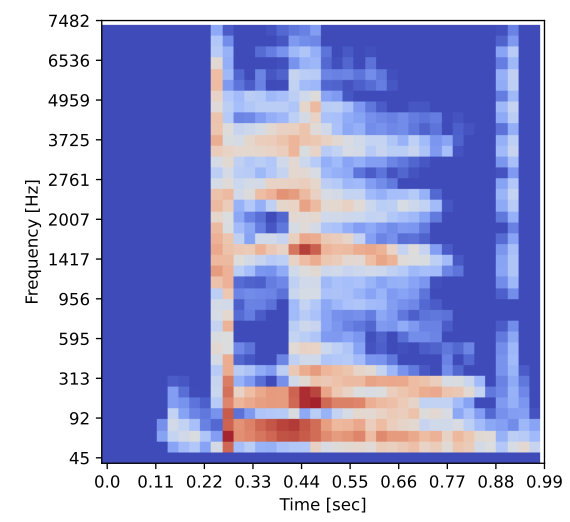
\includegraphics[width=\textwidth]{images/4.02 Spectrogram Edge Impulse.png}
        \caption{Edge Impulse Spectrogram}
    \end{subfigure}
    \hfill
    \begin{subfigure}[t]{0.5\textwidth}
        \centering
        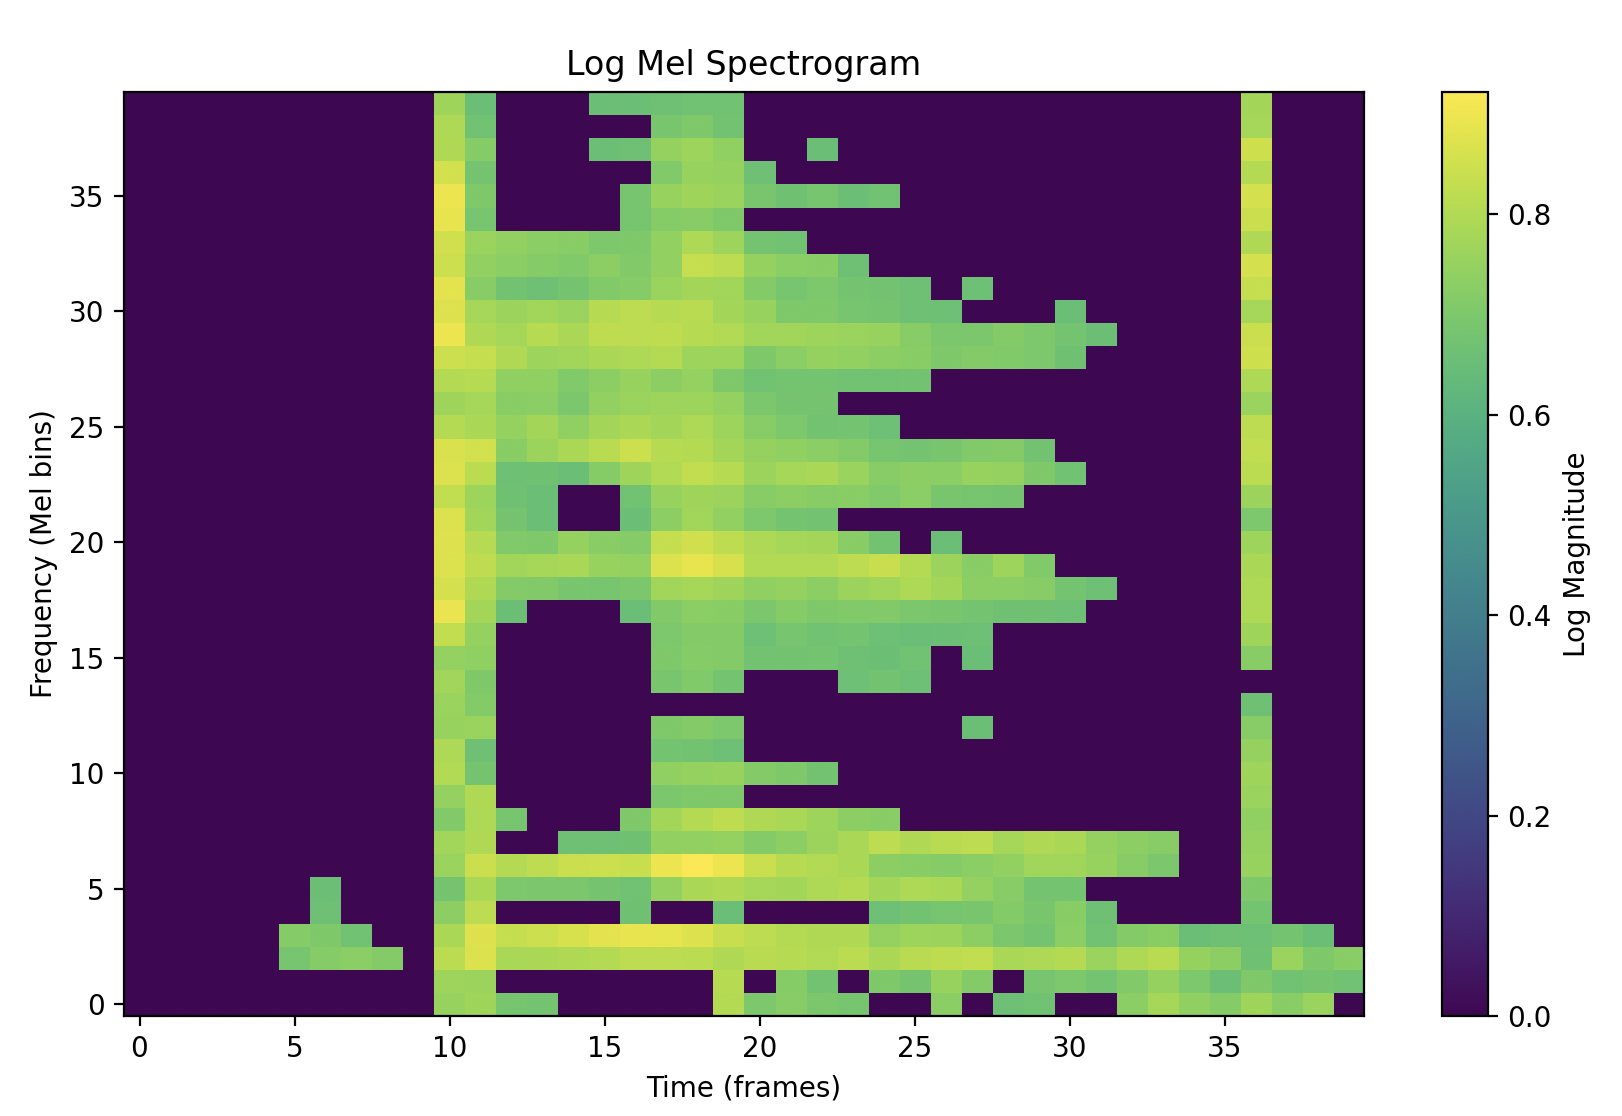
\includegraphics[width=\textwidth]{images/4.03 Spectrogram My Code.png}
        \caption{Custom Code Spectrogram}
    \end{subfigure}
    \caption{Comparison of Spectrograms}
\end{figure}

\begin{algorithm}[H]
\caption{Spectrogram Computation Pipeline}
\KwIn{Raw audio signal \texttt{audio[\,]} with \texttt{num\_samples} samples}
\KwOut{Log-Mel spectrogram \texttt{log\_mel\_spectrogram[\,]}}
\nl Normalize and apply pre-emphasis:\;
\Indp
    \For{$i \gets 0$ \KwTo $num\_samples - 1$}{
        $norm[i] \gets audio[i] / 32768.0$\;
    }
    $pre\_emphasis\_array[0] \gets norm[0]$\;
    \For{$i \gets 1$ \KwTo $num\_samples - 1$}{
        $pre\_emphasis\_array[i] \gets norm[i] - \texttt{COEFFICIENT} \times norm[i - 1]$\;
    }
\Indm
\nl Slice into overlapping frames and apply Hamming window:\;
\Indp
    \ForEach{frame $f$}{
        $fft\_in \gets$ frame of size \texttt{FRAME\_SIZE} from $pre\_emphasis\_array$\;
        \For{$i \gets 0$ \KwTo \texttt{FRAME\_SIZE} $- 1$}{
            $fft\_in[i] \gets fft\_in[i] \times (0.54 - 0.46 \times \cos(2\pi i / (FRAME\_SIZE - 1)))$\;
        }
\Indm
\nl Compute FFT and magnitude spectrum:\;
\Indp
        $fft\_out \gets \texttt{FFT}(fft\_in)$\;
        \For{$b \gets 0$ \KwTo \texttt{NUM\_BINS} $- 1$}{
            $spectrogram[f][b] \gets \sqrt{fft\_out[b].r^2 + fft\_out[b].i^2}$\;
        }
    }
\Indm
\nl Construct Mel filterbank:\;
\Indp
    Generate $FILTER\_NUMBER + 2$ evenly spaced Mel points between $MIN\_FREQ$ and $MAX\_FREQ$\;
    Convert Mel points to Hz and bin indices\;
    \ForEach{filter $j$}{
        Construct triangular filter between left, center, and right bins\;
        Assign weights to $mel\_filterbank[j][\,]$\;
    }
\Indm
\nl Apply Mel filters and compute log-Mel spectrogram:\;
\Indp
    \ForEach{frame $f$}{
        \ForEach{filter $j$}{
            $sum \gets \sum_k spectrogram[f][k] \times mel\_filterbank[j][k]$\;
            $log\_mel\_spectrogram[f][j] \gets 10 \times \log_{10}(sum + \varepsilon)$\;
        }
    }
\Indm
\nl Apply noise floor and quantization:\;
\Indp
    \ForEach{value in $log\_mel\_spectrogram$}{
        Normalize with respect to $NOISE\_FLOOR$\;
        Quantize to range $[0, 255]$, then normalize to $[0, 1]$\;
        Zero out values $< 0.65$\;
    }
\Indm
\KwRet{$log\_mel\_spectrogram$}
\end{algorithm}
\subsection{Models Processing}
The software pipeline first inferences the KWS model and according to the result, if major than 0, triggers SV one. In simulation, they are handled with the components of neural network explictly shown. To recall, shall be declared the weights and biases. At the same time, the input and output allocation of each layer should were allocated. Regarding the functions were created the fully connected layer process reasoning and the corresponding activation functions. The Syntiant model elaboration code for both KWS and SV models follow the following algorithm\footnotemark{}\footnotetext{Note that this is a general processing of a model, because in the case shown KWS performs a softmax needed for classification, but it is not mandatory for example SV performs only a ReLU. In the algorithm, is shown the KWS, but has to be adapted to user model needs.}, following the theoretical concepts.\newline
\begin{algorithm}[H]
\caption{Neural Network Inference Example}
\KwIn{Input vector $x \in \mathbb{R}^{\texttt{INPUT\_SIZE}}$}
\KwOut{Predicted class index $y$}

\textbf{Initialize:} \\
\Indp
Create hidden layer buffers:
$fc_1 \in \mathbb{R}^{H_1}, \;
fc_2 \in \mathbb{R}^{H_2}, \;
fc_3 \in \mathbb{R}^{H_3}, \;
output \in \mathbb{R}^{C}$ \;
\Indm

\textbf{Feedforward pass:} \\
\Indp
$fc_1 \gets \texttt{ReLU}(W_1 x + b_1)$ \;
$fc_2 \gets \texttt{ReLU}(W_2 fc_1 + b_2)$ \;
$fc_3 \gets \texttt{ReLU}(W_3 fc_2 + b_3)$ \;
$output \gets \texttt{ReLU}(W_4 fc_3 + b_4)$ \;
\Indm

\textbf{Softmax normalization (if classification needs):} \\
\Indp
$\texttt{softmax}(output)$ \;
\Indm

\textbf{Sort and classify:} \\
\Indp
Sort $output$ in descending order, track original indices \;
Print top-$C$ class probabilities and names \;
\Indm

\Return{index of class with highest score}
\end{algorithm}

\subsection{Output Processing}
After the model elaborates its output the result should take several directions, for KWS model classification method it consists simply in using the output class to perform the desired action, like triggering the SV model and can be simply done with a if-case in simulation and with SPI sending in inference, but different case is for SV model. To evaluate the result, it is used a cosine similarity approach, consisting in comparing two different reference d-vector finding a percentage of how much they are similar. Two different techniques of using reference features were explored in the previous chapter, but to compute the similarity has to be followed this mathematical formula, consisting in the scalar product of the two vectors long N, divided by the product of their euclidian norms:\newline
\begin{equation}
    cosine\_similarity(x,y)=\frac{x\cdot y}{|x|\cdot|y|}=\frac{\sum_{i=0}^{N}x_iy_i}{\sqrt{\sum_{i=0}^{N}x_i^2}\cdot\sqrt{\sum_{i=0}^{N}y_i^2}}
\end{equation}
This will do among reference samples using the techniques of bestmatching and mean-reference, previously introduced. So, after the comparison with the d-vector stored in the dataset according to the system threshold the result will be binary: 0, if it was not found a d-vector similar to the one given in input in the dataset, and 1, if yes.\newline
The structure of the dataset is first cataloged by words, then per user and, finally, per user's sample, if using benchmarking technique. This system is to simplify the overall computation reducing the number of reference d-vector to compare with the input one, simply giving the allocation in memory corresponding to the word selected and all the samples will be in a contiguous memory allocation to use spatial property, accessing only to the subsequent element and it uses an information that it should receive anyway. Another consideration is that if a samples receives a similarity above the threshold similarity the system exists directly and to output 0 it should parse all samples associated to the word given by KWS.\newline
\begin{center}
    \centering
    \begin{figure}[!h]
        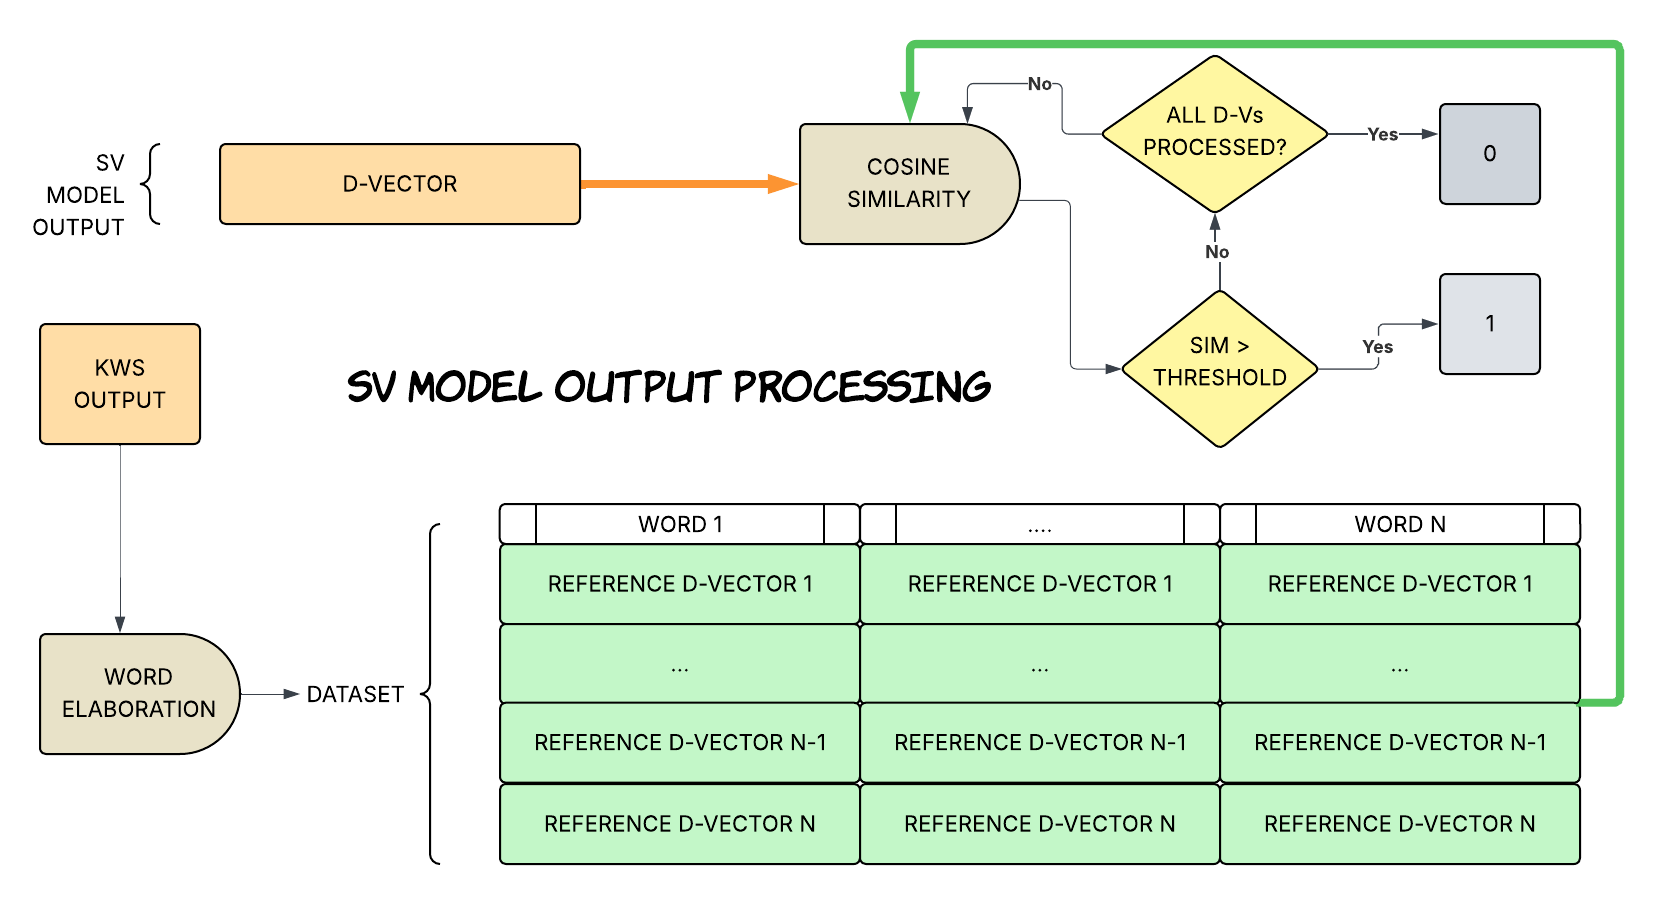
\includegraphics[width=1.0\textwidth]{images/4.04 D-Vector Processing.png}
        \caption{D-Vector Processing according to Database}
    \end{figure}
\end{center}
\subsection{Enrollment phase}
\label{subsec:enrollment} 
On inference, the complete application of this method is restricted due to the impossibility of quantizing the model to 4-bit precision and manipulating SPI interfaces. This limitation is primarily caused by the non-disclosure agreement (NDA) surrounding the Syntiant NDP101, which prevents direct control over its internal functions. The Speaker Verification (SV) model, however, was trained on a large and diverse dataset to generate a distinct d-vector representation for each user, thus enabling a one-time training process. In this scenario, the user needs to enroll by providing a number of voice samples. This number should be balanced: not too large to avoid excessive memory usage, but sufficient to maintain good recognition accuracy. The idea is to reuse the existing pipeline by replacing only the SV model’s inference stage. When enrolling, the user specifies the desired keyword, after which the system begins recording. However, it only saves samples that trigger the Keyword Spotting (KWS) model. Once the required number of valid samples is collected, the d-vectors are stored sequentially in memory by determining the current end of the dataset and appending the new d-vectors accordingly.
The memory structure for the dataset is designed such that each keyword is allocated a fixed portion of memory. Additionally, a separate structure tracks the number of samples collected per keyword. Since each d-vector has a fixed length, it becomes straightforward to calculate the memory offset for appending new vectors. In simulation, this dataset resides in a header file for simplicity, whereas in the actual inference phase, only the logic has been implemented—full system integration has not been completed due to the limitations in connecting with the KWS system on hardware. Ideally, the dataset would be stored directly in internal SRAM, taking into account its typical 256-byte size constraint. However, some microcontrollers (MCUs) support external SD card storage, which could be used as an alternative. Using a memory mapping technique to manage allocation could be effective even with larger memory sizes and is unlikely to significantly impact energy consumption. Nevertheless, internal storage is generally preferable and should be tailored based on the remaining available memory after code and global variable allocations. A best-matching approach, where multiple samples per user are stored and compared, typically yields higher accuracy but consumes more memory. Alternatively, averaging the d-vectors into a single representative vector per user results in lower precision but significantly reduces memory usage, as it eliminates the need for storing multiple individual vectors.
\section{Hardware Pipeline}
\label{sec:hw pipeline}
\subsection{Original System Implementation}
\begin{center}
    \centering
    \begin{figure}[!h]
        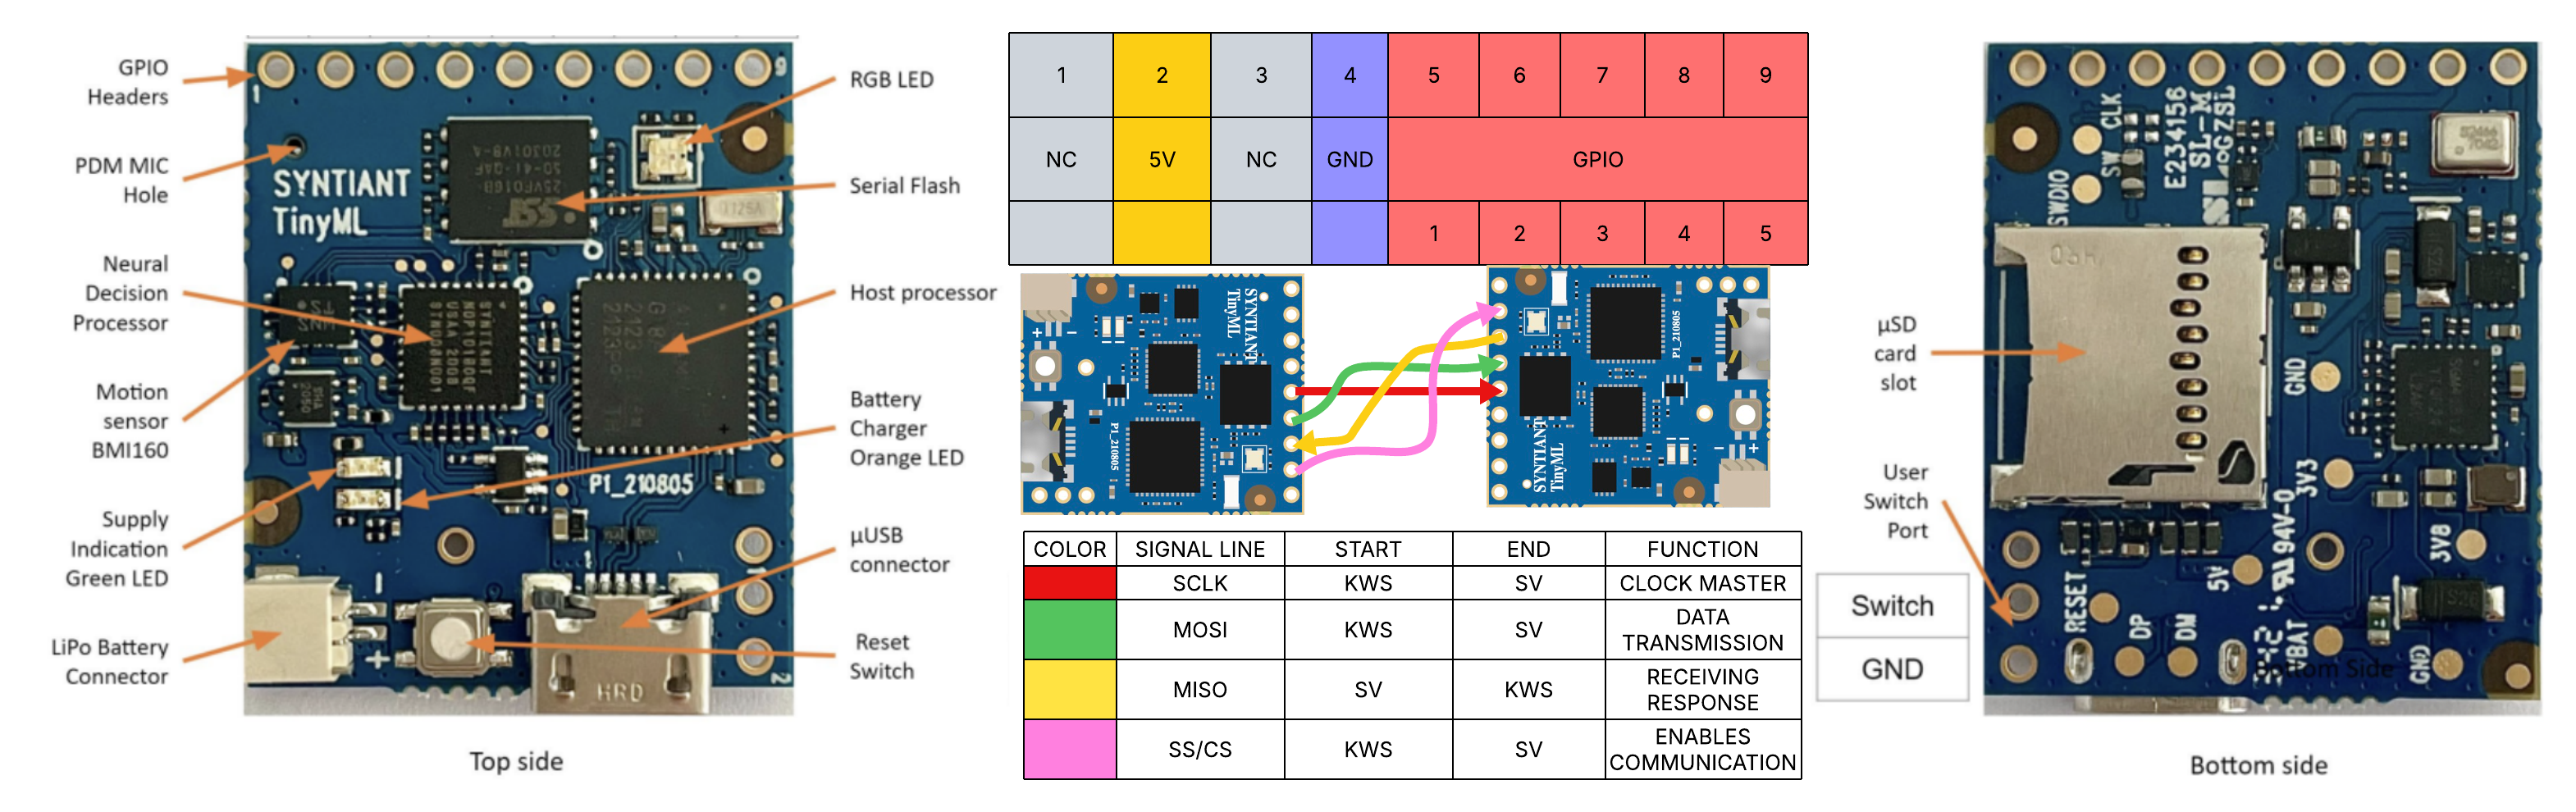
\includegraphics[width=1.0\textwidth]{images/4.05 Hardware Pipeline 2 NDP101.png}
        \caption{SV Model Output Processing}
    \end{figure}
\end{center}
The interaction of the system for 
• Structure of the system (2 Syntiant NDP101)\newline
-> SPI communication NDP101 + Arduino MKRZero\newline
-> SPI communication between ESP32 + NDP101\newline\newline
\newpage

PAGE 7
\newpage


